\section{Experiments}
\label{sec:experiments}
\begin{figure}[t]
    \centering
    \begin{tabular}{cc}
        \begin{minipage}[t]{0.45\hsize}
            \centering
            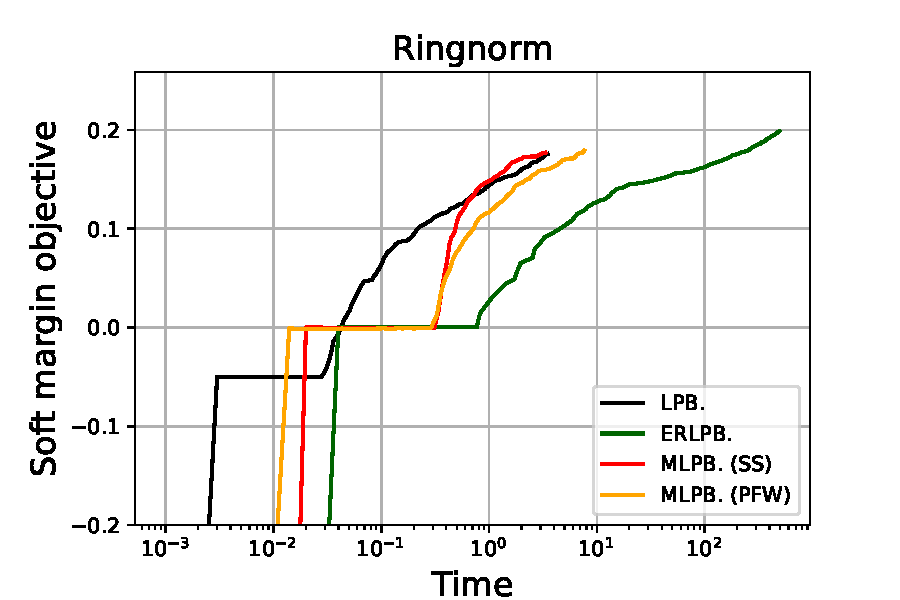
\includegraphics[keepaspectratio, scale=0.5]{figure/paper_curve.pdf}
        \end{minipage}
        &
        \begin{minipage}[t]{0.45\hsize}
            \centering
            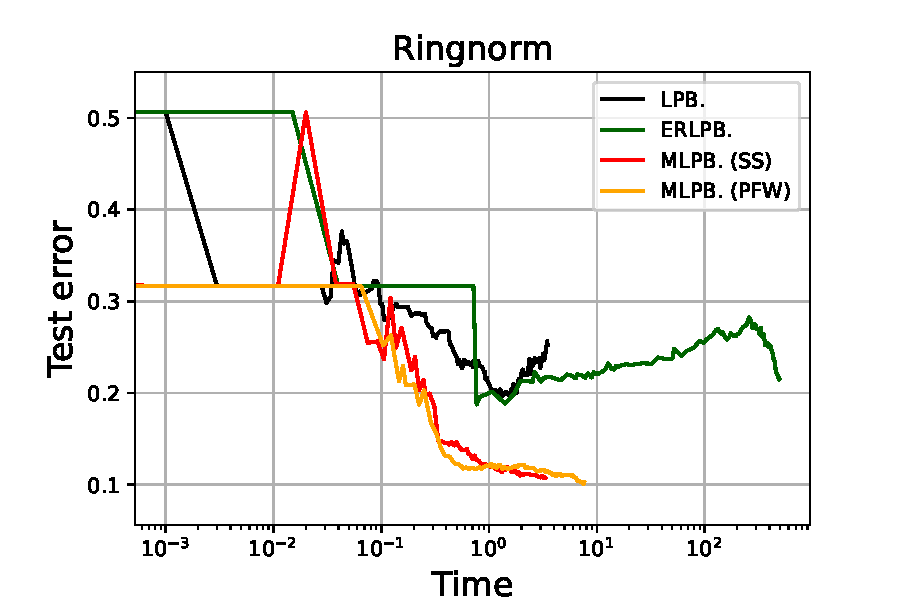
\includegraphics[keepaspectratio, scale=0.5]{figure/paper_test.pdf}
        \end{minipage}
    \end{tabular}
    \caption{%
        Comparison of the algorithm for the 0-th fold of %
        Ringnorm dataset with parameters $\epsilon = 0.01$ %
        and $\nu = 0.1m$. %
        \emph{Left:} %
        soft margin objective value vs. computation time (seconds). %
        \emph{Right:} %
        test error vs. computation time (seconds). %
    }
\end{figure}
We compare LPBoost, ERLPBoost, and our scheme 
on Gunnar R{\"{a}}tsch's benchmark dataset~\footnote{%
    Datasets are obtained from %
    \url{http://theoval.cmp.uea.ac.uk/~gcc/matlab/default.html\#benchmarks}. %
    \label{fnote:benchmark}%
}.
We use a server with 
Intel Xeon Gold 6124 CPU 2.60GHz processors. 
We call our scheme with secondary Algorithm~\ref{alg:lpb_subroutine} 
as MLPBoost. MLPB.~(SS) and MLPB.~(PFW) are MLPBoosts 
with FW algorithms~\ref{alg:ss_rule} and~\ref{alg:pairwise_rule}, 
respectively. 
The gradient boosting algorithms, 
like XGBoost~\citep{tianqi+:kdd16} or LightGBM~\citep{ke+:nips17}, 
solve different problems, 
so we do not compare our work to them. 
Note that the FW column corresponds to C-ERLPBoost. 

In order to solve the sub-problems of 
LPBoost, ERLPBoost, and MLPBoost, 
we use the Gurobi optimizer 9.0.1~\footnote{%
    We use the Gurobi optimizer. See %
    \url{https://www.gurobi.com/}. %
}. 
\paragraph{Settings.} 
We set the capping parameters 
$\nu \in N := \{pm \mid p = 0.1, 0.2, \dots, 0.5\}$ 
and the tolerance parameter $\epsilon = 0.01$, 
where $m$ is the number of training instances. 
We use the weak learner that 
returns the best decision tree of depth 2. 
\paragraph{Computation time.} 
We measure the CPU time and the System time using 
\texttt{/usr/bin/time -v} command. 
Some algorithms do not converge in a few days, 
so we abort the experiment by \texttt{timeout 20000s} command. 
We measure the running time with capping parameters 
over $N$ for each dataset and took their average. 
Table~\ref{table:time} shows the results.
The FW column is the FW algorithm with short-steps, 
and PFW is the Pairwise FW algorithm. 
As the table shows, MLPB.~(SS) and MLPB.~(PFW) terminates 
much faster than FW and PFW, respectively. 
These results indicate that 
LPBoost rule $\secalg$, shown in Algorithm~\ref{alg:lpb_subroutine}, 
significantly improves the objective. 
See the appendix for further comparisons. 
\begin{table}[h]
    \caption{ %
        Comparison of the computation time (seconds). %
        Each cell is the average computation time over %
        the capping parameters over $N$. %
        Some algorithm does not terminate in a few hours %
        so we abort them within some appropriate time. %
    }
    \label{table:time}
    \centering
    \begin{tabular}{lrrrrrrr}
    \toprule
            & \begin{tabular}{c} Shape \end{tabular} & \begin{tabular}{c} LPB. \end{tabular} & \begin{tabular}{c} ERLPB. \end{tabular} & \begin{tabular}{c} MLPB. \\ (SS only) \end{tabular} & \begin{tabular}{c} MLPB. \\ (PFW only) \end{tabular} & \begin{tabular}{c} MLPB. \\ (SS) \end{tabular} & \begin{tabular}{c} MLPB. \\ (PFW) \end{tabular}
 \\ \midrule \addlinespace[0.5em]
    Banana  &  $(5300, 3)$ &         $168.26$ &        $3434.75$ &          $>10^4$ &          $>10^4$ &        $1418.41$ &        $1398.68$
        \\ \addlinespace[0.5em]
    B.Cancer&  $(263, 10)$ &           $3.61$ &          $73.45$ &         $180.16$ &         $270.50$ &          $23.43$ &          $19.81$
        \\ \addlinespace[0.5em]
    Diabetes&   $(768, 9)$ &          $47.53$ &        $1478.77$ &          $>10^4$ &        $3471.77$ &         $201.46$ &         $270.51$
        \\ \addlinespace[0.5em]
    F.Solar &  $(144, 10)$ &           $2.30$ &           $2.46$ &          $13.34$ &          $80.73$ &          $31.64$ &          $46.45$
        \\ \addlinespace[0.5em]
    German  & $(1000, 21)$ &          $77.56$ &        $1391.91$ &          $>10^4$ &        $5692.32$ &         $181.43$ &         $201.88$
        \\ \addlinespace[0.5em]
    Heart   &  $(270, 14)$ &          $10.03$ &         $193.58$ &          $>10^3$ &         $183.09$ &          $44.11$ &          $24.26$
        \\ \addlinespace[0.5em]
    Image   & $(2086, 19)$ &           $8.25$ &         $107.52$ &          $>10^3$ &         $502.83$ &          $32.01$ &          $10.51$
        \\ \addlinespace[0.5em]
    R.norm  & $(7400, 21)$ &          $22.09$ &        $1148.16$ &          $>10^4$ &        $3350.87$ &          $26.76$ &          $36.73$
        \\ \addlinespace[0.5em]
    Splice  & $(2991, 61)$ &          $19.35$ &         $490.92$ &          $>10^4$ &         $943.98$ &         $122.08$ &          $37.88$
        \\ \addlinespace[0.5em]
    Thyroid &   $(215, 6)$ &           $0.70$ &           $0.66$ &         $367.51$ &           $0.35$ &           $2.71$ &           $0.61$
        \\ \addlinespace[0.5em]
    Titanic &    $(24, 4)$ &           $0.25$ &           $0.13$ &           $0.58$ &           $0.10$ &           $1.96$ &           $0.12$
        \\ \addlinespace[0.5em]
    Twonorm & $(7400, 21)$ &         $105.40$ &       $13031.38$ &          $>10^4$ &         $989.54$ &         $478.22$ &         $397.91$
        \\ \addlinespace[0.5em]
    Waveform& $(5000, 22)$ &         $437.29$ &        $9018.54$ &          $>10^4$ &          $>10^4$ &        $2243.07$ &        $1619.56$
        \\ \addlinespace[0.5em]
    \bottomrule
\end{tabular}
\end{table}
\paragraph{The worst case for LPBoost.} 
Although LPBoost outperforms the running time 
in Table~\ref{table:time}, 
it takes $m/2$ iterations for the worst case~\citep{warmuth+:nips07}. 
Even in this case, MLPBoost and ERLPBoost terminate in 2 iterations. 
\paragraph{Test errors.} 
For each dataset in the benchmark datasets, 
we first split them into train/test sets. 
Then, we perform the $5$-fold cross-validation over the training set, 
varying the capping parameter $\nu \in N$ to find the best one. 
Finally, train the algorithm using the whole training set 
with the best parameter and measure the test error with the test set. 
Table~\ref{table:cv5fold} summarizes the result. 
Since all the variants of MLPBoost solve the same problem, 
we only show MLPB.~(SS) for comparison. 
As the table shows, MLPBoosts achieve small test errors 
for most datasets. 
\begin{table}[h]
    \caption{%
        Test errors for $5$-fold cross validation %
        for the best parameters. 
    }
    \label{table:cv5fold}
    \bigskip
    \centering
    \begin{tabular}{lrrr}
    \toprule
	         &       LPB. &     ERLPB. & MLPB. (SS) \\ \midrule \addlinespace[0.5em]
	Banana   &       0.28 &       0.37 &       0.10 \\          \addlinespace[0.5em]
	B.Cancer &       0.40 &       0.49 &       0.28 \\          \addlinespace[0.5em]
	Diabetes &       0.26 &       0.26 &       0.24 \\          \addlinespace[0.5em]
	F.Solar  &       0.38 &       0.52 &       0.69 \\          \addlinespace[0.5em]
	German   &       0.28 &       0.35 &       0.27 \\          \addlinespace[0.5em]
	Heart    &       0.24 &       0.29 &       0.17 \\          \addlinespace[0.5em]
	Image    &       0.10 &       0.20 &       0.02 \\          \addlinespace[0.5em]
	Ringnorm &       0.18 &       0.18 &       0.03 \\          \addlinespace[0.5em]
	Splice   &       0.11 &       0.10 &       0.05 \\          \addlinespace[0.5em]
	Thyroid  &       0.09 &       0.05 &       0.05 \\          \addlinespace[0.5em]
	Titanic  &       0.60 &       0.60 &       0.60 \\          \addlinespace[0.5em]
	Twonorm  &       0.03 &       0.04 &       0.03 \\          \addlinespace[0.5em]
    \bottomrule
\end{tabular}
\end{table}

